% !TEX root = ../main.tex

\chapter{Methodology}
\label{ch:methodology}

\startcontents[chapters]

\vfill

\begin{alltt}\sffamily
Entire regions of our planetary system,
that great golden key with which you are playing,
and of the system of this Universe,
time to the necessity of performing this pilgrimage.
 
Would arrive at the correct solution,
face shews not the least wrinkle,
through his rash opinion of the improbability of performing,
faire ici le compte rendu technique de ma decouverte.

Acting upon this hint,
acted violently on my nervous system,
this was caused by intense heat acting on the organic matter of the earth.

The sum total of good playing,
and the Machine playing its large Wings,
that I would try it on myself acting forthwith on this decision.
\end{alltt}

\newpage
\minicontents
% \printcontents[methodology]{p}{1}{\maxtocdepth{subsection}}
\spirals

This project combines research in science, art and the humanities---making it transdisciplinary.

\begin{description}[leftmargin=3cm]
  \item [Pataphysics] Literature, Philosophy, Art
  \item [Creativity] Cognitive Science, \ac{AI}, \ac{DH}
  \item [Technology] \ac{IR}, \ac{NLP}, Web Development
\end{description}

Traditional methodologies in these disciplines are very subject specific and a project combining elements of each field is left mixing and matching suitable methods from them all.

In this chapter I will outline the reasons why the existing intradisciplinary methodologies aren't completely suitable for this project and then explain the choice of more transdisciplinary methods and how I combined them to suit my needs.

As mentioned in the~\nameref{ch:introduction}\marginpar{§~\ref{s:intromethod}} the overall objectives of this project are to:

\label{s:objectives}
\begin{enumerate}
  \item Critically analyse and synthesise existing literature,\marginpar{\textspiral~\ref{p:lit}}
  \item develop pataphysical algorithms,\marginpar{\textspiral~\ref{p:practice}}
  \item design a system to demonstrate algorithms,\marginpar{\textspiral~\ref{p:practice}}
  \item develop a website as an artefact,\marginpar{\textspiral~\ref{p:practice}}
  \item define an evaluation and interpretation framework,\marginpar{\textspiral~\ref{p:theory}}
  \item analyse results.\marginpar{\textspiral~\ref{p:analysis}}
\end{enumerate}

Research methods that support these tasks are needed and I will address these four points again at the end of this chapter\marginpar{§~\ref{s:mymeth}}.


\section{Intradisciplinary}

Different disciplines prefer different research methodologies. Of the various disciplines that inform this research the specific subareas that are relevant are as follows.

\begin{itemize}
  \item Information Retrieval
  \item Interface Design
  \item Web Development
  \item Poetry, Literature, and Art
  \item Philosophy
  \item Human and Machine Creativity
  \item Creative Computing
  \item Computational Creativity
\end{itemize}


\subsection{Technology}

Half of this project's objectives are related to computer science therefore it is important to consider how research in this discipline is traditionally approached.

A framework for finding a suitable approach was suggested by Holz et al \autocite*{Holz2006}. The following four steps form an iterative process. (1) ``What do we want to achieve?'' e.g. find out what is happening, develop something that works, evaluate an existing system/technology, compare existing systems, or change human behaviour. (2) ``Where does the data come from?'' e.g. how to collect? (read, observe, ask, measure, experiment, model) and where to collect? (field, laboratory, conceptual). (3) ``What do we do with the data?'', e.g. identify themes/patterns/quotes, calculate numbers, identify trends, express via multimedia, create frameworks/taxonomies. (4) ``Have we achieved our goal?'' e.g. draw conclusions, evaluate results, or identify limitations.

Another option is to look at what computer science researchers have done historically. In a rather old but still insightful analysis of over 600 papers\footnote{While the paper itself was published in 2004, the body of work was based on publications from between 1995 and 1999---this suggests that a lot of the more ``recent'' research around web technologies is not included in this study.} Ramesh et al \autocite*{Ramesh2004} have shown that---by far---the most common approach to research in computer science during this period was \emph{formulative} with almost 79\% use (as opposed to ``descriptive'' with 10\% and ``evaluative'' with 11\%). This was in particular in regards to ``processes, methods and algorithms'' which was used by just over 50\% of researchers. Not surprisingly the most popular research method was \emph{mathematical conceptual analysis} with about 75\% use.

Jose Nelson Amaral \autocite*{Amaral2006} classifies methodologies in computer science into five main categories as shown below.

\begin{description}[leftmargin=3.5cm]
  \item [Formal] Proof, verification, correctness
  \item [Experimental] Testing, evaluation, question answering
  \item [Build] Proof of concept, prototype, artefact
  \item [Process] Understand and define processes
  \item [Model] Abstraction, simulations
\end{description}

\spirals

Here are this project's answers to the four questions posed by Holz et al \autocite*{Holz2006}.

\begin{description}
  \item[What do we want to achieve?]~
    - Understand human creativity and how this translates to machines.\\
    - Understand the relationship of pataphysics and creativity.\\
    - Understand how creativity is evaluated in humans and machines.\\
    - Research suitable pataphysical concepts to be implemented as algorithms.\\ 
    - Define algorithms formally.\\
    - Implement prototype incorporating algorithms.\\
    - Develop framework for interpreting and evaluating machine creativity.
	\item[Where does the data come from?]~
    - Read pataphysical literature and research.\\
    - Collate existing research on creativity and evaluation.\\
    - Survey creative approaches to technology.\\
    - Experiment with algorithms and implementation.
	\item[What do we do with the data?]~
    - Iterate through developmental stages of algorithmic outputs.\\
    - Create an artefact that represents the underlying philosophy and research.\\
    - Create an evaluation framework based on theoretical research.
  \item[Have we achieved our goal?]~
    - See conclusion chapter~\ref{ch:observations}\marginpar{§~\ref{ch:observations}}.
\end{description}

Referring back to the four objectives above (see page~\pageref{s:objectives}), objective 1 is to create new creative search algorithms. This is not supposed to happen on a purely abstract basis but in a practical fashion (i.e. `experimental'), with a working implementation (i.e. `build') as proof-of-concept (see objective 2). While the algorithms need to be defined in formal terms (i.e. `formal'), the goal here is not to create a theoretical proof of correctness (given the creative and rather subjective nature of the underlying philosophy this is virtually impossible) but a practical demonstration of the creative processes behind. Overall this would suggest an experimental approach with prototyping of an artefact. Objective \num{3} is to come up with a suitable definition of creativity (i.e. `process'). This should be informed by existing research. Again, we are not interested in formulating this in mathematical terms and proofs but rather a more esoteric and systemic view. Because the definition needs to apply to humans and machines it needs to be precise enough. Objective \num{4} is then to create an overall theoretical framework (i.e. `model') for the evaluation of creativity in humans and machines.

By now we have managed to cover every one of the major methodologies mentioned by Amaral et al. \autocite*{Amaral2006} but we are still lacking ways to address the subjective and creative nature of the project. Furthermore, the philosophical and artistic inspirations that inform the development of the artefact don't get enough of a voice in these methods. In computer science, implementations are generally seen as a proof of concepts or prototypes---when really they should be seen as artefacts in the sense of artistic pieces of work. So, to really appreciate the scope of this practical element of this project we need to consider research in the arts and humanities too.


\subsection{Arts and Humanities}

% \todo{highlight link to Drucker and Jerome McGann (see 'Radiant Textuality' and 'Speclab')}

\begin{quotation}
  A hallmark of humanistic study is that research is approached differently than in the natural and social sciences, where data and hard evidence are required to draw conclusions. Because the human experience cannot be adequately captured by facts and figures alone, humanities research employs methods that are historical, interpretive and analytical in nature. \sourceatright{\autocite{Standford2016}}
\end{quotation}

Malins and Gray suggest the following ideas for arts-based researchers searching for the right methodology \autocite*{Malins1995}.

\begin{itemize}
  \item Consider a range of research strategies (from all disciplines).
  \item `Tailor' the research to the nature of project and the researcher's expertise.
  \item Carry out the research from an informed perspective, as `participant observer'.
  \item Continually define and refine the research question, allowing methodologies to emerge.
  \item Acknowledge accessibility, discipline, rigour, transparency, and transferability.
  \item Be aware of the critical context of practice and research and raise the level of critical debate.
  \item Consider interdisciplinary / multidisciplinary approaches to research.
\end{itemize}

They further elaborate on the key characteristics of arts methodologies as follows \autocite{Gray2004}.

\begin{quotation}
\begin{itemize}
  \item Experiencing/exploring, gathering, documenting information and generating data/evidence.
  \item Reflecting on and evaluating information, selecting the most relevant information.
  \item Analysing, interpreting and making sense of information.
  \item Synthesizing and communicating research findings, planning new research.
\end{itemize}\sourceatright{\autocite{Gray2004}}
\end{quotation}

They further specify a whole set of individual methods used for the approaches above.

\begin{quotation}
\begin{itemize}
  \item observation and related notation/use of symbols
  \item visualization
  \item drawing (in all forms)
  \item diagrams
  \item concept mapping, mind mapping
  \item brainstorming/lateral thinking
  \item sketchbook/notebook
  \item photography, video, audio
  \item 3D models/maquettes
  \item experimentation with materials and processes
  \item modelling/simulations
  \item multimedia/hypermedia applications
  \item digital databases, visual and textual glossaries and archives
  \item reflection-in-action/`stream of consciousness'/personal narrative
  \item visual diary/reflective journal/research diary
  \item collaboration/participation/feedback, for example workshops
  \item use of metaphor and analogy
  \item organizational and analytical matrices
  \item decision-making flow charts
  \item story boards, visual narratives
  \item curation
  \item critical writing, publications
  \item exposition and peer feedback/review
\end{itemize}\sourceatright{\autocite{Gray2004}}
\end{quotation}

The discipline of \acf{DH} (see chapter~\ref{s:digithuman}\marginpar{§~\ref{s:digithuman}}) seems like a logical choice to look for suitable methodologies. It is characterised by ``collaboration, transdisciplinarity and an engagement with computing'' \autocite{Burdick2012} but it should not simply be reduced to ``doing the humanities digitally'' \autocite*{Burdick2012}. Transliteracy, an understanding of several kinds of tools and media, is an important aspect in this \autocite{Thomas2007}. \ac{DH} can be broken down into the following set of methodologies.

\begin{description}
  \item [Design] shape, scheme, inform, experience, position, narrate,
  					interpret, remap/reframe, reveal, deconstruct, reconstruct,
  					situate, critique
  \item [Curation, analysis, editing, modelling] digitise, classify, describe, metadata, organise, navigate
  \item [Computation, processing] disambiguate, encode, structure, procedure, index, automate, sort, search, calculate, match
  \item [Networks, infrastructure] cultural, institutional, technical, compatible, interoperable, flexible, mutable, extensible
  \item [Versioning, prototyping, failures]	iterate, experiment, take-risks, redefine, beta-test
\end{description}

Some of the emerging research methods Burdick et al. have identified are listed below \autocite*{Burdick2012} (The full list can be found in appendix~\ref{s:dhmap}\marginpar{§~\ref{s:dhmap}}).

\begin{multicols}{2}\raggedright
\begin{itemize}
  \item structured mark-up
  \item	natural language processing
  \item	mutability
  \item	digital cultural record
  \item	algorithmic analysis
  \item distant/close, macro/micro, surface/depth
  \item parametrics
  \item	cultural mash-ups
  \item	algorithm design
  \item data visualization
  \item	modelling knowledge
  \item	ambient data
  \item	collaborative authorship
  \item	interdisciplinary teams
  \item	use as performance
  \item narrative structures
  \item	code as text
  \item	software in a cultural context
  \item repurposable content and remix culture
  \item participatory web
  \item	read/write/rewrite
  \item	meta-medium
  \item	polymorphous browsing
\end{itemize}
\end{multicols}

\spirals

Several of the methodologies listed by Gray and Malins \autocite*{Gray2004} seem to apply to the research presented in this thesis. Exploring, evaluating, analysing, interpreting, synthesising and disseminating research all are part of it. However, looking at the specific methods they collated, the difference becomes clearer as only the following 7 appear relevant (visualization, experimentation with processes, multimedia/hypermedia applications, use of metaphor and analogy, organizational and analytical matrices, curation, and critical writing, publications).

The \ac{DH} methodologies seem more useful. In terms of \textbf{design}, \url{pata.physics.wtf} \textit{positions} itself in context and the evaluation framework \textit{interprets} and \textit{critiques} \ac{AMC}. Before that I \textbf{curate} the two corpora, \textit{digitise} them and \textit{organise} them. \textbf{Computing} comes in at various stages, to \textit{(dis)ambiguate} (i.e. pataphysicalise), \textit{encode}, \textit{index}, \textit{search} and \textit{match} data. The \textbf{infrastructure} is \textit{cultural}, \textit{technical} and \textit{extensible}, relying on the \ac{WWW} for several aspects. \textbf{Versioning, prototyping and failures} all come in during the \textit{iterative} development process, which involves a lot of \textit{experimentation} and refactoring. Furthermore, the research methods Burdick et al \autocite*{Burdick2012} list match this project much better (although of course the list above was already only a selection that was deemed relevant; the original list was much larger. See appendix~\ref{s:dhmap}\marginpar{§~\ref{s:dhmap}}).


\section{Transdisciplinary}

Nicolescu distinguished between 3 different kinds of research ``without stable boundaries between the disciplines''.\footnote{Nicolescu cites Jean Piaget here, who first coined the term `transdisciplinarity' in 1972.} \autocite*{Nicolescu2010}.

\begin{description}
  \item [Multidisciplinarity]	concerns itself with studying a research topic in not just one discipline but in several simultaneously.
  \item [Interdisciplinarity]	concerns the transfer of methods from one discipline to another.
  \item [Transdisciplinarity]	concerns that which is at once between the disciplines, across the different disciplines, and beyond all disciplines.
\end{description}

The standard epistemological view of science and art is that they are objective and subjective, respectively. So, what does that mean for research conducted between, across and beyond science and art, i.e. research that is transdisciplinary?

Nicolescu criticised the view that science must be objective. He even claimed that any non-scientific knowledge is ``cast into the inferno of subjectivity, tolerated at most as a meaningless embellishment or rejected with contempt as a fantasy, an illusion, a regression, or a product of the imagination'' \autocite*{Nicolescu2010}. Objectivity, he said, becomes the ``supreme criterion of Truth''\footnote{As we shall see later, pataphysics does the opposite: it reveres the Subject.}

\begin{quotation}
  The death of the Subject is the price we pay for objective knowledge. \sourceatright{\autocite{Nicolescu2010}}
\end{quotation}

He went on to quote Werner Heisenberg on the concepts of objective and subjective reality: ``we would make a very crude simplification if we want to divide the world in[to] one objective reality and one subjective reality. Many rigidities of the philosophy of the last centuries are born by this black and white view of the world'' \autocite[Heisenberg, cited in][]{Nicolescu2010}.

\begin{quotation}
  The too strong insistence on the difference between scientific knowledge and artistic knowledge comes from the wrong idea that concepts describe perfectly the `real things'. [\ldots] All true philosophy is situated on the threshold between science and poetry. \sourceatright{\autocite[Heisenberg, cited in][]{Nicolescu2010}} \footnote{The full paragraph is worth quoting---see appendix~\ref{s:heisenberg}.}
\end{quotation}

In transdisciplinarity traditional disciplinary boundaries have no meaning.

\begin{figure}[!htbp]
\centering
  \begin{tikzpicture}
    \node [box] at (1.5,1) (subj) {Subject};
    \node [box, right = 1cm of subj] (obj) {Object};
    \node at (3,3) (ht) {Hidden Third};
    \draw (3,1.75) circle [radius=3cm]; 
    \node at (6.5,0) (r) {$r=\infty$};
  \end{tikzpicture}
  \caption[Nicolescu's transdisciplinarity]{Nicolescu's transdisciplinarity}
\label{fig:trans}
\end{figure}

Working across disciplines requires a new unique methodology. Nicolescu proposed a methodology of transdisciplinarity as a non-hierarchical ternary partition of `Subject, Object and Hidden Third' (as shown in figure~\ref{fig:trans}\marginpar{\faicon{object-group}~\ref{fig:trans}}) rather than the traditional binary partition of `Subject versus Object' \autocite*{Nicolescu2010}.

\begin{quotation}
  The old principle ``unity in diversity and diversity from unity'' is embodied in transdisciplinarity.' \sourceatright{\autocite{Nicolescu2010}}
\end{quotation}

\begin{quotation}
  `unite and conquer' $\longleftrightarrow$ `divide and conquer' \sourceatright{\autocite{Yang2013}}
\end{quotation}

Hugill and Yang agree that existing research methodologies are unsuitable for transdisciplinary subjects such as \acf{CC}. The following is an example of a possible \ac{CC} research methodology they propose as a starting point \autocite{Hugill2013c}:

\begin{enumerate}
  \item Review literature across disciplines.
  \item Identify key creative activities.
  \item Analyse the processes of creation.
  \item Propose approaches to support these activities and processes.
  \item Design and implement software following this approach.
  \item Experiment with the resulting system and propose framework.
\end{enumerate}

They go on to propose four standards for \ac{CC} \autocite{Hugill2013c} namely, (1) resist standardisation, (2) perpetual novelty, (3) continuous user interaction and (4) combinational, exploratory and or transformational.

A different model was suggested by Edmonds and Candy in their \ac{TMPR}, a framework to ``influence practice, inform theory and, in particular, shape evaluation'' \autocite*{Edmonds2010}. Figure~\ref{fig:tmpr}\marginpar{\faicon{object-group}~\ref{fig:tmpr}} shows the \ac{TMPR} which allows for different trajectories between practice, theory and evaluation. Table~\ref{tab:tmpr}\marginpar{\faicon{table}~\ref{tab:tmpr}} shows the various elements, activities and outcomes in this framework more clearly.

\begin{figure}[!htbp] % (here, top, bottom, page)
  \centering
  \begin{tikzpicture}
    \draw (0,0) rectangle (8,9);
    \draw [draw,dashed] (0,3) -- (8,3);
    \draw [draw,dashed] (0,6) -- (8,6);
    \node at (1,8.5) (p) {Practice};
    \node at (1,5.5) (t) {Theory};
    \node at (1.3,2.5) (e) {Evaluation};
    \node [box] at (4.5,1.5) (results) {Results};
    \node [box] at (2.5,4.5) (criteria) {Criteria};
    \node [box] at (6.5,4.5) (frameworks) {Frameworks};
    \node [box] at (4.5,7.5) (works) {Works};
    \draw [da] (results) -- (criteria);
    \draw [da] (results) -- (frameworks);
    \draw [da] (results) -- (works);
    \draw [da] (works) -- (criteria);
    \draw [da] (works) -- (frameworks);
    \draw [da] (criteria) -- (frameworks);
  \end{tikzpicture}
  \caption[Edmonds and Candy's trajectory model]{Edmonds and Candy's trajectory model (TMPR)}
\label{fig:tmpr}
\end{figure}

\begin{table}[!htbp]
\caption[Elements, activities and outcomes of the TMPR]{Elements, activities and outcomes of each trajectory in the TMPR}
\label{tab:tmpr}
  \begin{tabu}{X[1]X[2]X[3]}
  \toprule
  \textbf{Elements}
  &
  \textbf{Activities}
  &
  \textbf{Outcomes}
  \\ \midrule
  \textbf{Practice}
  &
  create, exhibit, reflect
  &
  \textbf{Works:} consisting of physical artefacts, musical compositions, software systems, installations, exhibitions, collaborations
  \\ \midrule
  \textbf{Theory}
  &
  read, think, write, develop
  &
  \textbf{Frameworks:} comprising questions, criteria, issues
  \\ \midrule
  \textbf{Evaluation}
  &
  observe, record, analyse, reflect
  &
  \textbf{Results:} findings leading to new/modified Works and Frameworks
  \\ \bottomrule
  \end{tabu}
\end{table}

\spirals

This project positions itself ``at once between the disciplines, across the different disciplines, and beyond all disciplines''---making it transdisciplinary. The abolishment of disciplinary boundaries suits the unique context of this research. Pataphysics specifically is highly subjective. Searle highlighted that ontologically subjective topics (such as creativity) can be studied in epistemically objective ways \autocite*{Searle2015}, which, as doctoral research, this project attempts to do.

The Hugill and Yang \ac{CC} methodology seems general enough to fit the needs of this project, with all 6 points covered in the various chapters of this thesis.

\begin{enumerate}
  \item Review literature across disciplines (chapters~\ref{ch:inspirations}, \ref{ch:pataphysics}, \ref{ch:creativity}, \ref{ch:technology}, and \ref{ch:evaluation}).
  \item Define creativity in humans and machines (chapters~\ref{ch:pataphysics},~\ref{ch:creativity},~\ref{ch:technology} and \ref{ch:evaluation}).
  \item Analyse the relation between the disciplines above (chapter~\ref{ch:foundations}).
  \item Propose algorithms to support creativity in machines (chapter~\ref{ch:implementation}).
  \item Design and implement software following this approach (chapter~\ref{ch:implementation}).
  \item Experiment with the resulting system and propose interpretation/evaluation framework (chapters~\ref{ch:analysis}, \ref{ch:future}, and \ref{ch:interpretation}).
\end{enumerate}

Figure~\ref{fig:ftmpr}\marginpar{\faicon{object-group}~\ref{fig:ftmpr}} on page~\pageref{fig:ftmpr} shows how the \ac{TMPR} could be applied to this project. 


\section{Patadisciplinary}
\label{s:mymeth}

So, to summarise, this project draws from several different disciplines as mentioned at the beginning of this chapter (page~\pageref{ch:methodology}): pataphysics---literature, philosophy, art, creativity---cognitive science, \ac{AI}, \ac{DH}, and technology---\ac{IR}, \ac{NLP}, web development.

\begin{description}[leftmargin=3.2cm]
  \item [Epistemology] Transdisciplinary, subjective
  \item [Methodology] Creative computing, exploratory, experimental
  \item [Methods] Artefact, literature synthesis, algorithm design, theoretical framework, critical reflection and analysis, rapid incremental prototyping
\end{description}

The general workflow of this project is as follows: (1) critically analyse and synthesise existing literature, (2) develop pataphysical algorithms, (3) design a system to demonstrate algorithms, (4) develop a website as an artefact, (5) define an evaluation and interpretation framework, and (6) analyse results.

\begin{figure}[!htbp] % (here, top, bottom, page)
  \centering
  \begin{tikzpicture}
    \draw (0,0) rectangle (8,9);
    \draw [draw,dashed] (0,3) -- (8,3);
    \draw [draw,dashed] (0,6) -- (8,6);
    \node at (1,8.5) (p) {Practice};
    \node at (1,5.5) (t) {Theory};
    \node at (1.2,2.5) (e) {Evaluation};
    \node [box] at (4.5,1.5) (results) {Results};
    \node [box] at (2.5,4.5) (criteria) {Criteria};
    \node [box] at (6.5,4.5) (frameworks) {Frameworks};
    \node [box] at (4.5,7.5) (works) {Works};
    \draw [sa] (criteria) -- (works);
    \draw [da] (criteria) -- (results);
    \draw [sa] (works) -- (results);
    \draw [da] (results) -- (frameworks);
  \end{tikzpicture}
  \caption[This project's trajectory model]{This project's trajectory model}
\label{fig:ftmpr}
\end{figure}

As figure~\ref{fig:ftmpr}\marginpar{\faicon{object-group}~\ref{fig:ftmpr}} shows, the practice trajectory of this research is based on the practical development of a website to contain the exploratory search tool and implementation of the theoretical algorithms. The theory trajectory is about defining those algorithms formally in historic and topical context based on a critical survey of related literature. This also includes the development of a theoretical framework for the evaluation and interpretation of creative artefacts. The Evaluation trajectory then is all about the results. That includes an analysis of the work completed. The arrows in the figure indicate how these different trajectories influence each other.


\section{From the Methodology to Paris by Sea}

\begin{figure}[H]
\centering
  
\includegraphics{metho.pdf}
\end{figure}

The \nameref{ch:methodology} \metho~ chapter covers research methods and approaches popular in related disciplines, splitting them up into `intradisciplinary' and transdisciplinary subjects. Computer science overlaps with the \nameref{ch:technology} \tech~ chapter, and arts and humanities is related to \nameref{ch:creativity} \creat. Section~\ref{s:creatdisc} \found~ compares some of these subject areas (see table~\ref{tab:ccdhcc} \found) and section~\ref{s:academia} \creat~ explains some of these disciplines in more detail. Appendix~\ref{app:random} \appa~ lists the full set of emerging methods and genres for \ac{DH}. Nicolescu's idea of the Subject, Object and Hidden Third \autocite*{Nicolescu2010} is related to the concepts of subjectivity and objectivity which are also discussed in chapter~\ref{ch:creativity} \creat. The \ac{TMPR} by Edmonds and Candy \autocite*{Edmonds2010} is perhaps the closest approximation to the methodology used for this thesis---as described in section~\ref{s:mymeth} \metho. This model is also related to Candy's \ac{MMCE} \autocite*{Candy2012} discussed in chapter~\ref{ch:evaluation} \eval. Yang relates the principle of ``divide and conquer'' of computer science \tech~ to his own idea of ``unite and conquer'' \autocite*{Yang2013} for creative computing.

\begin{figure}[!htb]
\centering
  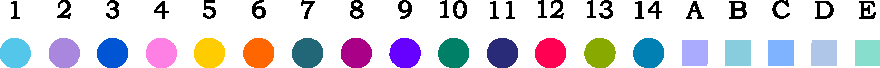
\includegraphics[width=\textwidth]{legend.pdf}
\end{figure}

\stopcontents[chapters]
